%%%%%%%%%%%%%%%%%%%%%%%%%%%%%%%%%%%%%%%%%%%%%%%%%%%%%%%%%%%%%%%%%%%%%%%%%%%%%%%%%%%%%%%%%%
%
%	LAN\c{C}ADORES ESPACIAIS/SPACE LAUNCHERS, GROUP 5 PROJECT REPORT
%	INPUTS FOR THE MAIN FILE
%	AUTHORS: 			SIMONE BINOTTO, MARCO AZEVEDO, PHILIPPE QUICHAUD, CORENTIN OUISSE
%	AUTHORS:			ANDRE MATOS, THEO DEMESY
%	INITIAL CODING:		01/3/2025
%	LAST UPDATE:		12/3/2025
%%%%%%%%%%%%%%%%%%%%%%%%%%%%%%%%%%%%%%%%%%%%%%%%%%%%%%%%%%%%%%%%%%%%%%%%%%%%%%%%%%%%%%%%%%






\documentclass[3p,preprint,12pt]{elsarticle}	% review, preprint, 5p



%%%%%%%%%%%%%%%%%%%%%%%%%%%%%%%%%%%%%%%%%%%%%% PACKAGES AND COMMANDS INCLUDED BY AUTHORS

\usepackage{siunitx}                %SI units
\usepackage{tikz}                   %Figures (Drawings)
\usepackage{caption}
\usepackage{subcaption}
%\usepackage{commath}
%\usepackage[utf8]{inputenc}
\usepackage{float}                  %To use H and force flots "here"
\usepackage{booktabs}
\usepackage{url}
\usepackage{amsthm}
\usepackage{amssymb}
\usepackage[intlimits]{amsmath}

\usepackage{graphicx}
\usepackage{color}

\usepackage{natbib}				% para ter as refs no texto para confirma\c{c}\~{a}o

%%%%%%%%%%%%%%%%%%%%%%%%%%%%%%%%%%%%%%%%%%%%%%%%%%%%%%%%%%%%%%%%%%%% Def.
%%%%%%%%%%%%%%%%%%%%%%%%%%%%%%%%%%%%%%%%%%%%%%%%%%%%%%%%%%%%%%%%%%%%%%%%%%%%%%%%%%%%%%%%%%
%
%	LAN\c{C}ADORES ESPACIAIS/SPACE LAUNCHERS, GROUP 5 PROJECT REPORT
%	INPUTS FOR THE MAIN FILE
%	AUTHORS: 			SIMONE BINOTTO, MARCO AZEVEDO, PHILIPPE QUICHAUD, CORENTIN OUISSE
%	AUTHORS:			ANDRE MATOS, THEO DEMESY
%	INITIAL CODING:		01/3/2025
%	LAST UPDATE:		12/3/2025
%%%%%%%%%%%%%%%%%%%%%%%%%%%%%%%%%%%%%%%%%%%%%%%%%%%%%%%%%%%%%%%%%%%%%%%%%%%%%%%%%%%%%%%%%%

\newcommand{\CourseNamePt}{Lan\c{c}adores Espaciais}		% course name in Portuguese
\newcommand{\CourseNameEng}{Space Launchers}			% course name in English
\newcommand{\YearDegree}{1st year, MEAer}				% year in degree, degree

\newcommand{\AcademYear}{2025/26}

\newcommand{\VersionDoc}{\textcolor{blue}{1.0}}		% version of the document; see abstract

\newcommand{\maxGroupsize}{\textcolor{blue}{5}}		% max and ideal group size

\newcommand{\ProjectDeadline}{\textcolor{blue}{30th March, 2026, 23:59 (Monday, last week of classes})}	% project deadline

\newcommand{\ProjectPresentation}{\textcolor{blue}{8th April, 2026, 14:00--18:00 (Wednesday, week before exams})}	% project deadline

\newcommand{\PresentDuration}{\textcolor{blue}{10~min}}	% presentation duration

\newcommand{\PresentDiscussion}{\textcolor{blue}{20~min}}	% discussion duration

\newcommand{\MaxPages}{\textcolor{blue}{20}}	% max number of pages of the report






  % some command definition, see input.tex file


\theoremstyle{definition}		% To define the topics style
\newtheorem{topic}{Topic}		% To define the topics environment

\newcommand{\dd}{\ensuremath{\text{d}}}
\newcommand{\arcsinh}{\ensuremath{\text{arcsinh}}}
\newcommand{\arccosh}{\ensuremath{\text{arccosh}}}

\newcommand{\mma}{Mathematica\textsuperscript{\tiny\textregistered}}
%%% 	defining command for frequent symbols can be advantageous, especially if you think the symbol definition can change; but don't exaggerate; journal don't like it and beware of command definition collisions
%\newcommand{\mma}{Mathematica\textsuperscript{\tiny\textcopyright}}	
\newcommand{\matlab}{MATLAB\textsuperscript{\tiny\textregistered}}

\newcommand{\topicsep}{\vspace{0.4cm}}

\biboptions{sort&compress}

%%%%% To Create a Nomenclature
%\usepackage{framed} % Framing content
%\usepackage{multicol} % Multiple columns environment
%\usepackage{nomencl} % Nomenclature package
%\makenomenclature
%\setlength{\nomitemsep}{-\parskip} % Baseline skip between items
%\renewcommand*\nompreamble{\begin{multicols}{2}}
%\renewcommand*\nompostamble{\end{multicols}}
%% Group variables according to their symbol type
%\RequirePackage{ifthen}
%\renewcommand{\nomgroup}[1]{%
%    	\ifthenelse{\equal{#1}{A}}{%
%    		\item[\textbf{Acronyms}]}{%
%      \ifthenelse{\equal{#1}{R}}{%
%        \item[\textbf{Roman symbols}]}{%
%        \ifthenelse{\equal{#1}{G}}{%
%          \item[\textbf{Greek symbols}]}{%
%          \ifthenelse{\equal{#1}{S}}{%
%            \item[\textbf{Subscripts}]}{%
%            \ifthenelse{\equal{#1}{T}}{%
%              \item[\textbf{Superscripts}]}{}}}}}}%
%

%%%%%%%%%%%%%%%%%%%%%%%%%%%%%%%% PACKAGES E FUN\c{C}\~{O}ES de TRABALHO --- APAGAR QUANDO SUBMETER

%\usepackage[pdftex,usenames,dvipsnames*,svgnames,rgb]{xcolor} % Enabling colors by their 'svgnames'
\usepackage[color=blue!20!white,linecolor=red,figcolor=white,textwidth=1.9cm,colorinlistoftodos,%
textsize=scriptsize]{todonotes}		% op\c{c}\~{o}es:	disable,

\newcommand{\fazer}[1]{\colorbox{yellow}{\textbf{#1}}}	% yellow box

%\usepackage{showkeys}				% op\c{c}\~{o}es: 	[notref,notcite]


\usepackage{lineno}
%\linenumbers	% op\c{c}\~{o}es: \linenumbers 	ou \begin{linenumbers}... \end{linenumbers}
\modulolinenumbers[5]

\usepackage[hyperfootnotes=false, hyperfigures=true,colorlinks=false, pdfborder={0 0 0}]{hyperref}			% op\c{c}\~{o}es a confirmar, apenas as copiei, conv\'{e}m hyperref ser das \'{u}ltimas a carregar, com excep\c{c}\~{o}es
%\renewcommand{\sectionautorefname}{\S}	% para usar \autoref em vez de \ref e n\~{a}o aparecer Se\c{c}\~{a}o
%\renewcommand{\subsectionautorefname}{\S}	% para usar \autoref em vez de \ref e n\~{a}o aparecer Se\c{c}\~{a}o
%\renewcommand{\subsubsectionautorefname}{\S}	% para usar \autoref em vez de \ref e n\~{a}o aparecer Se\c{c}\~{a}o

%%%%%%%%%%%%%%%%%%%%%%%%%%%%%%%%%%%%%%%%%%%%%%%%% FIM DE PACKAGES AND COMMANDS INCLUDED BY AUTHORS

\usepackage[capitalise,sort&compress]{cleveref}		% must be loaded after hyperref


\graphicspath{{./figs/}}


\journal{\CourseNamePt, \YearDegree}

%%%%%%%%%%%%%%%%%%%%%%%
%% Elsevier bibliography styles
%%%%%%%%%%%%%%%%%%%%%%%
%% To change the style, put a % in front of the second line of the current style and
%% remove the % from the second line of the style you would like to use.
%%%%%%%%%%%%%%%%%%%%%%%

%% Numbered
%\bibliographystyle{model1-num-names}

%% Numbered without titles
%\bibliographystyle{model1a-num-names}

%% Harvard
%\bibliographystyle{model2-names.bst}\biboptions{authoryear}

%% Vancouver numbered
%\usepackage{numcompress}\bibliographystyle{model3-num-names}

%% Vancouver name/year
%\usepackage{numcompress}\bibliographystyle{model4-names}\biboptions{authoryear}

%% APA style
%\bibliographystyle{model5-names}\biboptions{authoryear}

%% AMA style
%\usepackage{numcompress}\bibliographystyle{model6-num-names}

%% `Elsevier LaTeX' style
\bibliographystyle{elsarticle-num}
%%%%%%%%%%%%%%%%%%%%%%%

% Fix problem with appendix names; see https://tex.stackexchange.com/questions/26333/elsarticle-appendix-and-a-table-of-contents
\renewcommand*{\appendixname}{}

\begin{document}

\begin{frontmatter}

\title{{\Large \CourseNamePt \tnoteref{mytitlenote} (\YearDegree )}\\
{\large Academic Year \AcademYear}\vspace{.5cm}\\
Project Report - Electric Propulsion
}
\tnotetext[mytitlenote]{\CourseNameEng .}


%% Authors in the order of appearance on Fenix page
\author[LEA-ist-address]{Simone Binotto ist116780\corref{group}}
\cortext[group]{Group \#\num{5}}
\ead{simone.binotto.2@studenti.unipd.it} 

\author[LEA-ist-address]{Marco Azevedo ist88166}
\ead{marco.azevedo@tecnico.ulisboa.pt}

\author[LEA-ist-address]{Philippe Quichaud ist119295}
\ead{philippe.quichaud@tecnico.ulisboa.pt}

\author[LEA-ist-address]{Corentin Ouisse ist119278}
\ead{corentin.ouisse@tecnico.ulisboa.pt}

\author[LEA-ist-address]{Andr\'{e} Matos ist106376}
\ead{andre.f.matos@tecnico.ulisboa.pt}

\author[LEA-ist-address]{Th\'{e}o Demesy ist119525}
\ead{theo.demesy@tecnico.ulisboa.pt}

\address[LEA-ist-address]{LEAer, Instituto Superior T\'{e}cnico, Universidade de Lisboa, Av. Rovisco Pais, 1049-001 Lisboa, Portugal}


\begin{abstract}
	This document is the report of Group \#\num{5} for the project in \emph{\CourseNamePt} (\CourseNameEng) in the Academic Year \AcademYear. The authors worked on subject 11, Electric propulsion. This is \textcolor{blue}{Version \VersionDoc} of this document.
\end{abstract}

\begin{keyword}
propulsion \sep electric \sep space hardware \sep performances
%\MSC[2010] 00-01\sep  99-00
\end{keyword}



\end{frontmatter}

%\linenumbers

%%% NOMENCLATURA - VER COMENT SE FOR NECESS\'{A}RIA, SE N\~{A}O, APAGAR NA VERS\~{A}O A SUBMETER

%	Nas regras da Acta Astronautica refere que a nomenclatura deve estar no fim do artigo, ap\'{o}s os ap\^{e}ndices, e que deve existir um rodap\'{e} na p\'{a}gina onde aparecem pela primeira vez a indicar "See Nomenclature at end of paper."
%\input{nomenc}

\setcounter{tocdepth}{2}
\tableofcontents

\newpage

\section{Introduction}

\subsection{State of the art}
    Chemical propulsion offers the significant advantage of generating high thrust levels, which are essential for rocket launch and the insertion of spacecraft into orbit. However, once in orbit, it is legitimate to question whether these propulsion methods remain the most efficient option.

The energy delivered by chemical combustion is intrinsically linked to the mass of propellant available on board. This dependence introduces a major limitation: increasing the available energy requires additional propellant mass, yet accelerating this extra mass demands even more energy, leading to a compounding cycle.

As a result, this strong mass dependence fundamentally constrains the performance of chemical propulsion systems, particularly their specific impulse, which is typically limited to an upper bound on the order of 500 seconds (\cite{mtp_book} p.652).

We will see that this limit can be overcome thanks to electric propulsion.

\subsection{Scope and Objectives}
The purpose of this report is to study and compare five existing electric propulsion systems currently used in industry. These technologies are based on three fundamental physical principles: electrostatic, electrothermal, and electromagnetic propulsion (\cite{mtp_book} p.651).

For each technology, this report presents the underlying physical principles, its practical implementation, and key performance parameters such as thrust ($F$), specific impulse ($I_{sp}$), exhaust velocity ($u_e$), and efficiency ($\eta$). Finally, a comparative analysis is conducted to highlight the advantages, limitations, and typical applications of each technology.
\section{Electrothermal Thrusters}

\subsection{Introduction}

Electrothermal propulsion comprises all techniques whereby a propellant gas is heated electrically and then expanded through a nozzle to convert its thermal energy to a jet of directed kinetic energy. In this chapter we shall consider two substantially different electrical means for heating the propellant flow:
\begin{enumerate}
    \item by passing it over an electrically heated solid surface, the so-called \textit{resistojet};
    \item by passing it through an arc discharge, usually termed an \textit{arcjet}.
\end{enumerate}
In each case we shall find that the attainable exhaust velocity is determined primarily by the maximum temperature that the chamber and nozzle surfaces can tolerate and by the gas-kinetic and thermodynamic properties of the propellant gas (\cite{pep_book} p. 90).

\subsection{Performances}

The gross performance of accelerators of this class can be forecast by reference to a general conceptual model. Electrical power from an external supply of given capacity $P$ is delivered in some manner to heat a propellant stream in a suitable chamber to some maximum temperature $T_c$. The electrically heated gas is then allowed to expand through a supersonic nozzle to a low pressure determined by the nozzle area ratio and by the chamber pressure $P_c$ (\cite{pep_book} p. 91).

Under the assumptions of one-dimensional adiabatic constant specific heat expansion through the nozzle, the attainable exhaust speed $u_e$ may be written from a simple energy balance \cite{pep_book} p. 91):
\begin{equation}
    \frac{1}{2} u_e^2 + C_p T_e = C_p T_{0c}
\end{equation}
By substituting the isentropic flow relations into the energy balance equation, we obtain the standard expression for the exit velocity:
\begin{equation}
    u_e = \sqrt{\frac{2\gamma}{\gamma-1} \frac{R_o T_c}{\mathcal{M}} \left[ 1 - \left( \frac{p_e}{p_c} \right)^{\frac{\gamma-1}{\gamma}} \right]}
\end{equation}

Assuming that the expansion is infinite where exit pressure is zero, the equation becomes:
\begin{equation}
    u_e = \sqrt{2 C_p T_c}
\end{equation}

The constant-pressure specific heat of the propellant gas per unit mass $C_p$ is seen to be a particularly critical quantity, since it defines the stagnation enthalpy which can be imparted to the gas at a given temperature, and thereby limits the attainable exhaust velocity (\cite{pep_book} p. 91).

Other parameters that characterize the performance of electrothermal thrusters are: thrust coefficient $C_F$, characteristic velocity $C^*$, specific impulse $I_{sp}$, and various efficiencies, as used in chemical rocket engines. The specific impulse $I_{sp}$ can be related to thrust coefficient $C_F$ and characteristic velocity $C^*$, as given in the following:
\begin{equation}
    I_{sp} = \frac{C_F C^*}{g_0}
\end{equation}

Note that the characteristic velocity $C^*$ does not depend on the method of heating of the propellant gas, which can be observed from the following expression:
\begin{equation}
    C^* = \sqrt{ \frac{1}{\gamma}{\frac{R_o T_c}{\mathcal{M}}}{\left( \frac{\gamma+1}{2} \right)^{\frac{\gamma+1}{\gamma-1}}} }
\end{equation}

In electrothermal rockets, the characteristic velocity $C^*$ depends only on the molecular weight, specific heat ratio, and temperature of propellant gas as in the case of chemical rocket (\cite{fund_rocket_prop} p. 407). 

Now that we have defined the characteristic velocity, we can say that the mass flow rate $\dot{m}$ through the nozzle can be as follows:
\begin{equation}
    \dot{m} = \frac{p_c A_t}{C^*}
\end{equation}
The relation for choked mass flux can be easily obtained by substituting Equation (5) in Equation (6) as follows:
\begin{equation}
    \dot{m} = \frac{p_c A_t}{\sqrt{T_c}}\sqrt{\frac{\gamma}{\frac{R_o}{\mathcal{M}}}\left(\frac{2}{\gamma+1}\right)^{\frac{\gamma+1}{\gamma-1}}}
\end{equation}

The last important equation is about the thrust $F$, that we can express as:
\begin{equation}
    F = \dot{m} u_e + (p_e - p_a) A_e
\end{equation}
where the first and second terms represent the momentum contribution and pressure components of thrust, respectively. The maximum thrust can be obtained only when the nozzle exhaust pressure is equal to the ambient pressure ($p_e = p_a$):
\begin{equation}
    F_{max} = \dot{m} u_e
\end{equation}

The nonideality of an electrothermal accelerator can be catalogued by defining the partial efficiency with which electric energy is delivered from the source to heat the gas stream, $\eta_h$; the aerodynamic, or nozzle, efficiency with which the stream follows a one-dimensional adiabatic route through the expansion process, $\eta_a$; and the efficiency with which it converts internal energy in the propellant stream to directed kinetic energy, $\eta_f$. 

As such, $1-\eta_h$ accounts for losses in the heating process; $1-\eta_a$ covers the nozzle viscous and profile losses; $1-\eta_f$ describes the unrecovered internal energy in the exhaust jet, often called frozen flow losses. It is essential that the overall thruster efficiency $\eta = \eta_h \eta_a \eta_f$ be kept high if the complete electrothermal propulsion system is to retain its advantage over chemical rockets (\cite{pep_book} p. 93).



\section{Resistojets}

\subsection{Principles}
The resistojet is the simplest of all electrical thrusters, consisting of an electrically heated pressure chamber and a convergent–divergent nozzle similar to the chemical rocket engine. In this case, the propellant gas is heated by making it come into contact with an electrically heated solid surface (\cite{fund_rocket_prop} p. 405).
Some of the heating elements for resistojets are shown in Figure 1.
\begin{figure}[H]
    \centering
    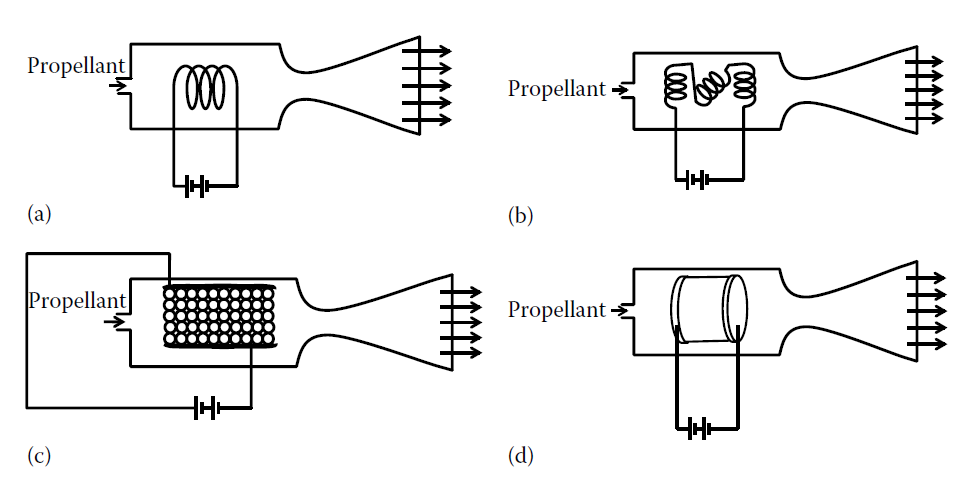
\includegraphics[width=0.5\linewidth]{figs/resistojet_pic1.png}
    \caption{Four types of electrical heating elements for resistojets: (a) straight coiled wire, (b) transverse coiled wire, (c) sphere bed, and (d) chamber wall.}
    \label{resistojet_schematics}
\end{figure}

In the case of straight coiled wire resistojet, propellant passes along the heating element, which restricts the heating rate of the propellant. In order to improve the heating rate of the propellant, heating coils can be placed in transverse direction of flow. A bed of tungsten spheres is used to heat the propellant by passing current through the contact resistances of spheres. However, it enhances the bulkiness while incurring significant pressure losses. 

The performance of such kind of resistojets depends on the extent of heat transfer from resistance element to the propellant gas stream and radiative heat transfer from the complete assembly as heat loss through the walls is basically a loss of power in the thruster (\cite{fund_rocket_prop} p. 406).

\subsection{Energy Balance}
The electrical energy is transformed into heat. This is defined as the Joule heating effect. The theoretical heat can be calculated using the following energy balance equation:
\begin{equation}
    P_{elec} = I^2 R = \dot{m} C_p (T_c - T_{in}) + \dot{Q}_{loss}
\end{equation}
For ideal heating, electrical energy equals heat energy (\cite{resjet} p. 165). We can define the heat transfer efficiency $\eta_h$, so we can rewrite the energy balance as:
\begin{equation}
    \eta_h P_{elec} = \dot{m} C_p (T_c - T_{in})
\end{equation}

A design objective in resistojets is to keep heat losses in the chamber low relative to the power consumed. This can be done by: (1) the use of external insulation; (2) internally located radiation shields; (3) entrant flow layers or cascades.
Another important reason for heat-isolation is to keep any stored propellant from overheating under all operating conditions (\cite{Sutton2016-RPE9th} p. 633).

In the case of a chemical rocket, temperature of propellant gas is dependent on the propellant composition and not on its mass flow rate. In contrast, in the electrothermal rocket, temperature is dependent inversely on the mass flow rate:
\begin{equation}
    T_c \propto \frac{P_{elec}}{\dot{m}}
\end{equation}

For a fixed power, if the mass flow rate is too small for a particular heat input, then the temperature may rise to spoil the heating element itself. Hence, an electrothermal thruster has a maximum flow rate/power ratio that is limited by the materials of filaments and chamber wall (\cite{fund_rocket_prop} p. 407).

Electrical energy can be lost due to (1) wasted electrical power (stray currents, ohmic resistances, etc.), (2) heat losses, (3) nonaxial component of exhaust, and (4) nonuniform heating of propellant (\cite{fund_rocket_prop} p. 408). 

The thruster efficiency $\eta$ can be defined as the ratio of the kinetic energy rate producing the thrust of the exhaust nozzle to the total electrical power, given as follows:
\begin{equation}
    \eta = \frac{\dot{m}u_e^2}{VI} = \frac{FI_{sp}g_o}{2VI}
\end{equation}
where $V$ is the voltage and $I$ is the current. Generally, the thruster efficiency of resistojets varies from 65\% to 90\% (\cite{fund_rocket_prop} p. 408).

\subsection{Specific Characteristics}
The highest specific impulse has been achieved with hydrogen (because of its lowest molecular mass), but its low density makes propellant storage too bulky (cryogenic storage is unrealistic for most space missions). Since virtually any propellant is appropriate, a large variety of different gases have been used,  such as $H_2O$, $CO_2$, $NH_3$, $CH_4$ and $N_2$ (\cite{Sutton2016-RPE9th} p. 633).

The major engineering problems of designing and developing resistojets is the fabricating and maintaining of the conducts and insulators that can keep electrical integrity and vacuum seals at high temperature in the range of 2500–3000 K (Mishra, 2017, p. 408). Resistojets are fundamentally temperature-limited by the available structural materials, which at present constrain them to a range of exhaust velocities below $10^{-4} \text{ m/s}$ and a maximum possible specific impulse of about 300 sec for typical storable propellants; however, resistojets that use hydrogen can go beyond 800 sec
(\cite{pep_book} p. 110).
 
Resistojet thrusters typically produce low thrust levels (10--200 mN, up to 1 N) with mass flow rates between $10^{-6}$ and $10^{-4}$ kg/s.
In spite of low values of thrust and mass flow rate, these thrusters are preferred for space applications. They are deployed for auxiliary but important applications during satellite operation, station keeping, drag neutralization, attitude control, and so on, where compactness, high reliability, and low thrust are called for (\cite{fund_rocket_prop} p. 409).
\section{Arcjets}

\subsection{Principles}

Arcjets constitute a branch of propulsion technology under the electrothermal electrical rocket propulsion heading. AS such, to generate thrust, the propellant is heated and forced trough a typical convergent-divergent nozzle. Heat is transferred to the propellant using an electric arc induced by a high current discharge. As stated in \cite{rpe_book}, the physical components of the system are relatively simple, as opposed to the phenomenology they explore: \textit{plasma physics}. The electric effect requires cathode and anode elements. These requirements are solved by typically placing the cathode as a centered element inside the nozzle, with the nozzle shell serving itself as the anode element.

\begin{figure}[h]
    \centering
    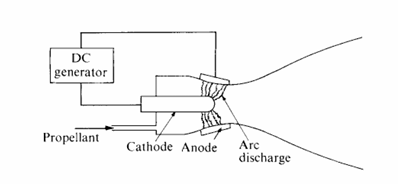
\includegraphics[width=0.5\linewidth]{figs/arcjet_pic1.png}
    \caption{Schematic diagram of an arcjet \cite{mtp_book}}
    \label{arcjet_schematics}
\end{figure}

The largest differentiator of this technology is the ability to achieve heating temperatures much higher than surrounding walls, overcoming the fundamental limitation of \textit{Resistojet Rocket Propulsion} systems.


\subsection{Electric Subsystem}

All the arcjet working architecture assume the successful generation of an electric arc. As the propellants, in the chamber, are a gaseous medium, electricity conduction trough it requires that a certain ionization threshold is achieved. This effect is analogous to a lightning discharge. Overall, this process is inherently unstable, \cite{agr_book}, thus consisting in the most difficult stage of arcjet propulsion systems. To stabilize the electrical arc, a constrictor design  with tangential propellant injection is often employed, to induce a swirl inside the nozzle. This also helps with cooling and preserving the nozzle material. \cite{pep_book}

A sensible approach for the plasma physics is to consider the gaseous medium as uniform. Applying the generalized Ohm's Law, the propellant is subject to Ohmic heating. \cite{rpe_book}

\begin{equation}
\label{eq:ohm_1}
    V = IR = \left( \frac{I}{A} \right) \left( \frac{AR}{d} \right) (d)
\end{equation}

Equation \eqref{eq:ohm_1} assuming the very same uniform medium, the electric field is $E = V / d$, current density $j = I/A$ and \textit{electrical conductivity} as $\sigma = d / AR$. The electrical conductivity is proportional to \textit{free electrons} \cite{rpe_book}. 

The ionization level useful to the process depends on: High temperatures and/or low ionization threshold requirements. To help kickstart the effect, the gases may be pre-processed by \textit{seeding} them with low ionization potential vapors. The plasma conductivity can be calculated regarding the free electrons motion.


\begin{equation}
\label{eq:sigma_condut}
    \sigma = \frac{e^2n_e\tau}{\mu_e} 
\end{equation}

In reality, arc currents are influenced by magnetic fields,  further detailed models exist to represent the phenomena. \cite{rpe_book}. If constant conductivity $\sigma$ si assumed, the volumetric power input can be computed as \cite{pep_book}:

\begin{equation}
\label{eq:arcjet_pele_comp}
    P_e = j \cdot E = \sigma E^2
\end{equation}

To start and arcjet thruster, an initial higher voltage discharge is employed to disrupt the cold gas and induce plasma production. After that, the steady-state arc is preserved and conditioned with resistance or ballast mechanism. \cite{rpe_book}

Downstream the arc, the propellant is partially ionized into a plasma, a enthalpy rich state, of mainly thermal and ionization energy. The further expansion over the nozzle provides the conversion into the desired kinetic energy.

\subsection{Mathematical Model}

As stated in the previous chapter, arcjet modeling requires the coupling of both fluid dynamics and electromagnetic principles.

Narrowing down the envelope of operation to free space (vacuum), thrust can be derived from the momentum balance of the nozzle outer boundary:

\begin{equation}
\label{eq:arcjet_thrust}
    F = \dot{m} u_e
\end{equation}

With specific impulse:

\begin{equation}
\label{eq:isp_arcjet}
    I_{sp} = \frac{u_e}{g_0} =\frac{F}{\dot{m} g_0}
\end{equation}

Thruster efficiency is given by the ratio between the power of jet and the power input:

\begin{equation}
\label{eq:arcjet_eff_1}
    \eta_T = \frac{power \ of \ the \ jet}{overall \ power \ input}
\end{equation}

Depending on the propellant used and system architecture, the input power may be all electrical, or a combination of electrical and chemical energy, as in hydrazine decomposition \cite{rpe_book}. With $P_e = electric \ power$,generalized ohms law, $P_{chem} = chemical \ power$ and $P_{in} = power \ input$:

\begin{equation}
\label{eq:pchm_arcjet}
    P_{chem} = \dot{m} \ h_{chem}
\end{equation}

\begin{equation}
\label{eq:pi_arcjet}
    P_{in} = P_e + P_{chem} 
\end{equation}

The power generated on the thruster results from the kinetic energy rate seen at the nozzle exhaust \cite{rpe_book}: 

\begin{equation}
\label{eq:pj_arcjet}
    P_{j} = \frac{1}{2} \dot{m} u_e^2 =  \frac{1}{2} \dot{m} \left( \frac{F}{\dot{m}} \right)^2 = \frac{F^2}{2 \dot{m}}
\end{equation}

Replacing \eqref{eq:pj_arcjet} and \eqref{eq:pi_arcjet} into \eqref{eq:arcjet_eff_1}:

\begin{equation}
\label{eq:arcjet_eff_2}
    \eta_t = \frac{P_j}{P_{in}} = \frac{\frac{1}{2} \dot{m}u_e^2}{P_e + P_{chem}} = \frac{\frac{1}{2} \frac{F}{I_{sp} g_0} \left( I_{sp} g_0 \right)^2}{P_e + P_{chem}} = \frac{1}{2} \frac{F I_{sp} g_0}{{P_e + P_{chem}}}
\end{equation}

For scenarios where chemical energy is meaningless, the efficiency if further simplified into:

\begin{equation}
\label{eq:arcjet_eff_3}
    \eta_t = \frac{F I_{sp} g_0}{2 P_e}
\end{equation}

Combining $P_j$ with $P_in$, $\eta_t$ and $I_{sp}=$ \cite{fep_book}, the system can be expressed as $u_e$ \eqref{eq:arcjet_ue} or $I_{sp}$ \eqref{eq:arcjet_isp}:

\begin{equation}
\label{eq:arcjet_ue}
    \eta_t = \frac{\frac{1}{2} \dot{m}u_e^2}{P_{in}} \Leftrightarrow u_e = \sqrt{\frac{2 \eta_t P_e}{\dot{m}}} 
\end{equation}


\begin{equation}
\label{eq:arcjet_isp}
    \eta_t = \frac{\frac{1}{2} \dot{m}u_e^2}{P_{in}} \Leftrightarrow u_e = \sqrt{\frac{2 \eta_t P_e}{\dot{m}}} \Leftrightarrow I_{sp} = \frac{1}{g_0} \sqrt{\frac{2 \eta_t P_e}{\dot{m}}}
\end{equation}

\subsection{Specific Characteristics}

For current technology,  only roughly half of the energy can be converted into useful kinetic energy. Up to 20 \% is wasted as heat, via dissipation and radiation, with the remaining fraction representing the residual energy and ionization present on the plume. This effect, frozen flow, results from the dissociation of molecules due to the electric arc and inability to recombine in the nozzle due to the very fast flow.  At the same time, the cathode suffers erosion, aggravated by power cycling. This contributes to an additional loss of efficiency over the lifespan of the thruster.\cite{mtp_book}


%\begin{table}[H]
%\centering
%\caption{Typical Performance Parameters of Arcjet Propulsion Systems \cite{rpe_book}}
%\label{tab:arcjet_performance}
%\begin{tabular}{@{}ll@{}}
%\toprule
%\textbf{Parameter} & \textbf{Typical Value} \\ \midrule
%Thrust Range (mN) & 200 -- 1000 \\
%Specific Impulse (sec) & 400 -- 800 \\
%Thruster Efficiency (\%) & 30 -- 50 \\
%Thrust Duration & Months \\
%Typical Propellants & $H_2$, $N_2$, $N_2H_4$, $NH_3$ \\
%Kinetic Power per Unit Thrust (W/mN) & 2-3 \\ \bottomrule
%\end{tabular}
%\end{table}

\section{Ion Thrusters}

\subsection{Operating Principles}

Ion thrusters are electrostatic devices that achieve high exhaust velocities by decoupling ionization from acceleration, entirely removing the thermodynamic limits of electrothermal systems. Operation occurs in three sequential stages: ionization, electrostatic acceleration, and beam neutralization. Inside a positively biased discharge chamber, a hollow cathode emits electrons that bombard neutral propellant (typically xenon) to form positive ions. These ions drift toward the ion optics—a highly positive screen grid and a negative accelerator grid—which extract and axially accelerate the beam \cite{fep_book}. Finally, a downstream neutralizer cathode injects electrons into the exhaust to prevent spacecraft charging \cite{holste_2020}. 

\begin{figure}[htb]
    \centering
    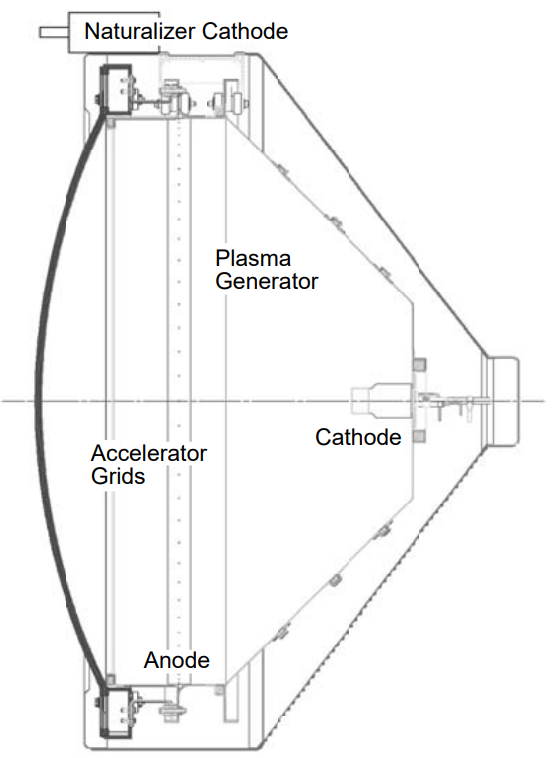
\includegraphics[width=0.25\textwidth]{figs/ion_thrusters_1.png}
    \caption{Cross-section of a gridded ion thruster (electron bombardment type) \cite{fep_book}}
    \label{fig:git_schematic}
\end{figure}

%A notable variant is the radio-frequency ion thruster (RIT), which replaces the internal cathode with an RF coil for inductive plasma heating, thereby eliminating cathode erosion and extending lifespan \cite{holste_2020}.

\subsection{Propellant Selection}

Propellant selection balances high atomic mass, low ionization energy, chemical inertness, and storability \cite{dietz_2019}. Xenon (131.3~amu, 12.13~eV) offers the best compromise and remains the industry standard \cite{fep_book, dietz_2019}. Krypton is increasingly used in commercial constellations (e.g., Starlink) to reduce costs, despite requiring higher jet power for equivalent thrust \cite{holste_2020}. Legacy propellants like cesium and mercury are obsolete due to toxicity and spacecraft contamination.

\begin{table}[htb]
\centering
\caption{Properties of selected ion thruster propellant candidates \cite{dietz_2019, fep_book}}
\label{tab:ion_propellants}
\begin{tabular}{@{}llll@{}}
\toprule
\textbf{Propellant} & \textbf{Atomic/Mol.} & \textbf{1st Ionization} & \textbf{Status} \\
                    & \textbf{Mass (amu)}  & \textbf{Energy (eV)}    &                 \\ \midrule
Xenon (Xe)   & 131.3 & 12.13 & Industry standard \\
Krypton (Kr) & 83.8  & 14.00 & Commercial (Starlink) \\
Iodine (I)   & 126.9 & 10.45 & Research / CubeSat \\
Cesium (Cs)  & 132.9 & 3.89  & Obsolete (toxic) \\
Indium (In)  & 114.8 & 5.79  & FEEP micro-thrusters \\ \bottomrule
\end{tabular}
\end{table}

\subsection{Performance Equations}

\subsubsection{Exhaust Velocity \& Thrust}

An ion of charge $q$ and mass $M$ accelerated through a net potential difference $V_b$ gains kinetic energy, defining the exhaust velocity \cite{holste_2020}:

\begin{equation}
\label{eq:ion_ve}
    v_e = \sqrt{\frac{2 q V_b}{M}}
\end{equation}

where $q = e = 1.602 \times 10^{-19}$~C for singly charged ions. Thrust is the momentum flux of the accelerated beam \cite{fep_book}:

\begin{equation}
\label{eq:ion_thrust}
    T = \dot{m} \, v_e = I_b \sqrt{\frac{2 M V_b}{q}}
\end{equation}

While inherently low-thrust (e.g., NSTAR produces 20--90~mN at 2.3~kW), continuous operation over months accumulates massive $\Delta v$ with minimal propellant \cite{holste_2020}.

\subsubsection{Specific Impulse}

Specific impulse ($I_{sp} = v_e/g_0$) routinely reaches 1500--10\,000~s in flight-qualified GIEs, far exceeding chemical limits \cite{holste_2020}. By the Tsiolkovsky equation:

\begin{equation}
\label{eq:tsiolkovsky}
    \Delta v = I_{sp} \, g_0 \ln\left(\frac{m_0}{m_f}\right)
\end{equation}

this high $I_{sp}$ yields exceptionally favorable mass ratios. For $\Delta v > 5$~km/s, chemical propulsion becomes practically infeasible, making ion propulsion an enabling technology \cite{holste_2020}.

\subsubsection{Efficiency Metrics}

Thruster performance is primarily characterized by mass utilization ($\eta_m$) and overall thruster efficiency ($\eta_T$). \textbf{Mass utilization efficiency} captures the fraction of admitted propellant that is ionized and accelerated \cite{holste_2020}:

\begin{equation}
\label{eq:ion_massutil}
    \eta_m = \frac{\dot{m}_i}{\dot{m}_p} = \frac{I_b M}{e \dot{m}_p}
\end{equation}

\textbf{Thruster efficiency} is the ratio of jet power to total electrical input power ($P_{in}$) \cite{holste_2020, fep_book}, which expands directly into its constituent sub-efficiencies:

\begin{equation}
\label{eq:ion_eff}
    \eta_T = \frac{T^2}{2 \dot{m}_p P_{in}} = \eta_e \eta_m \xi^2
\end{equation}

where $\eta_e$ is the \textbf{electrical efficiency} (fraction of input power successfully converted to beam power) and $\xi$ is the \textbf{thrust correction factor} accounting for beam divergence and multiply-charged ions. %A key secondary metric is the \textbf{ion production cost} $\eta_d = P_d / I_b$, representing the discharge power spent per ion \cite{holste_2020}. For GIEs, this amounts to several hundred eV---well above xenon's ionization threshold---constituting the dominant internal loss mechanism.

\subsection{Specific Characteristics and Limitations}

Grid erosion from charge-exchange (CEX) collisions is the primary wear mechanism, limiting operational lifetime to roughly 10,000--100,000 hours. During CEX, fast extracted ions interact with neutral propellant to create slow secondary ions that are drawn back to sputter the negatively biased accelerator grid \cite{holste_2020}. Operationally, thrusters are heavily constrained by electrical power; inverse-square solar power losses eventually necessitate nuclear sources for deep-space missions. Furthermore, the supply of xenon—a rare byproduct of air liquefaction—is a growing bottleneck. Rising prices driven by mega-constellations have rapidly accelerated research into cheaper alternatives like krypton and iodine \cite{holste_2020, dietz_2019}.

%\begin{table}[htb]
%\centering
%\caption{Typical performance parameters of gridded ion thrusters \cite{holste_2020, fep_book}}
%\label{tab:ion_performance}
%\begin{tabular}{@{}ll@{}}
%\toprule
%\textbf{Parameter} & \textbf{Typical Value} \\ \midrule
%Thrust Range             & 0.01~mN -- 750~mN \\
%Specific Impulse         & 1\,500 -- 10\,000~s \\
%Exhaust Velocity         & 15 -- 100~km/s \\
%Thruster Efficiency      & 30 -- 90\% \\
%Thrust-to-Power Ratio    & 20 -- 250~mN/kW \\
%Input Power              & 0.1 -- 20~kW \\
%Typical Propellants      & Xe, Kr, I$_2$ \\
%Operational Lifetime     & Years \\ \bottomrule
%\end{tabular}
%\end{table}
\section{Hall Thrusters}

\subsection{Working principles}

Hall Thrusters are a purely electric propulsion technology. As stated in \cite{fep_book}, they share the propulsive mechanism with ion thrusters: the propellant, usually Xenon, is ionized and accelerated through an electric field to provide thrust. However, the ionization process differs from a grid-based ion-thruster: the technology uses the eponym Hall-effect to capture a dense plasma of free electron through which the neutral propellant jet passes. This allows for a more compact and simpler design than ion thrusters, but often at the cost of efficiency and specific impulse.

\begin{figure}[H]
    \centering
    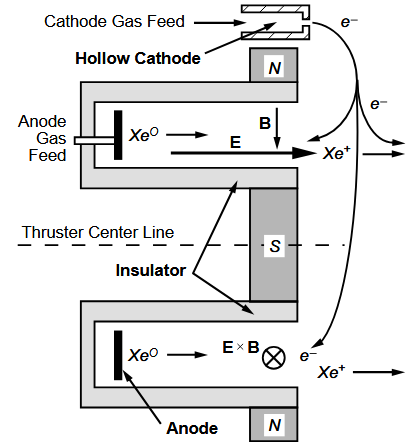
\includegraphics[width=0.3\linewidth]{figs/hall_thrusters_1.png}
    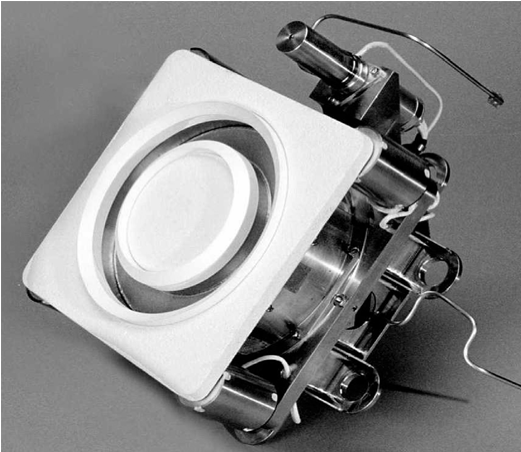
\includegraphics[width=0.3\linewidth]{figs/hall_thrusters_2.png}
    \caption{Left, a schematic of an Hall thruster. Right, an Hall thruster manufactured by Aerojet \cite{fep_book}}
    \label{het_illustration}
\end{figure}

The circular ring where the reaction takes place is called the channel. Magnets and an iron shunt are used to generate a strong radial magnetic field while an anode/cathode pair generates a longitudinal electric field. The cathode has two aditionnal roles: providing electrons for the plasma in the channel and jet neutralization.

The main advantage of this technology is that it isn't burdened by the charge limiting effect of standard ion thrusters and is therefore not space limited. Indeed, the propellant is  neutral throughout most the channel and is ionized only at the end of it, where the trapped electron plasma lies.

\subsection{The use of electromagnetic field}

As explained in \cite{demo_het}, the whole idea of an Hall thruster is to exploit the mass difference between electron ($9.109 \cdot 10^{-31}$kg) and ions (usually on the order of $10^{-26}$kg) so that the two particles have a different behaviour in the channel. Namely, ions are simply accelerated through the channel by the electric field and ejected to provide thrust while the electrons are captured by the magnetic field to generate the ionization plasma. Applying Newton first law to all of these particle, subjected to electromagnetic forces:

\begin{equation}
\label{eq:het_newton}
    m\vec{a} = q\vec{E} + q\vec{v}\times\vec{B}
\end{equation}

It follows that a charged particule tends to be accelerated along electric field lines and orbit magnetic field lines. The orbit radius, commonly refered as the Larmor radius, can be calculated as such, where $E_c$ is the kinetic energy of the particle:

\begin{equation}
\label{eq:het_larmor}
    r = \frac{\sqrt{2mE_c}}{qB}
\end{equation}

Considering only the effect of engine-generated electromagnetic field and not particle to particle interactions for simplification, it is posible calculate the two Larmor radius of electrons and ions. Since the radius depends on mass, the relation $r_e << r_i$ is generally verified. Hall thrusters are functional on the condition $r_e << l_c << r_i$, where $l_c$ is the length of the channel. Using cheap magnets whith peak field of 0.0270T, \cite{demo_het} found a Lamor radius of 0.33mm for electrons and 20m for ion, which allows for a comfortable dimensionning of the channel.

Under this condition, electrons are circling at the end of the channel and form a current (called Hall current), bombarding the passing ions, eventually ionizing some by collision. These ions are then ejected by the eletric field, providing thrust. Electrons will then either traverse the channel and close the circuit by contact with the anode or also be ejected.

\subsection{Efficiency}

The exhaust velocity of Hall Thrusters is simply $v_e = \sqrt{2eV_A/m_i}$, where $V_A$ is the acceleration voltage and $\dot{m_i}$ the mass flowrate of ions. The thrust efficiency is then, with $P$ the consumed electric power and $\dot{m_p}$ the mass flowrate of propellant:

\begin{equation}
\label{eq:het_threff}
    r = \frac{\sqrt{\dot{m_p}v_e^2}}{2P}
\end{equation}

Hall thrusters rely deeply on a efficient and quick ionization process in the channel. Denoting $N_a$ the density of neutral propellant in the plasma region of the channel, it appears that $N_a(z) = N_{a0}\exp(-z/L_i)$, where $L_i$ is the caracteristic length of ionization. Generally, this length shall be really small compared to the length of the channel. The length can be related to electron temperature $T_e$, electron density $n_e$ and speed of electron along the azimuth $u_{az}$, all of them derivable from operating parameters through plasma physics:

\begin{equation}
\label{eq:het_ionlen}
    T_e^{3/2} \sim \frac{L_i n_e}{u_{az}}
\end{equation}

The main power loss from an Hall Thruster comes from electrons in the Hall current colliding with the channel walls, eroding it and diminishing power of the Hall current. This power loss can be approximated trough, with $A_w$ the walls area:

\begin{equation}
\label{eq:het_wallloss}
    P_w \sim T_e^{3/2} n_e A_w
\end{equation}

%\subsection{Typical performances}

%This table is an extract from table 4.10 of \cite{nasa_report} and reports performances of the EDB Fakel SPT-50 Hall thruster (Russian thruster installed on Canopus-V). Refer to the source material for more example and details. As most of electric propulsion systems, Hall thrusters present a very high specific impulse (generally a bit higher than 1000s) but a poor thrust (in the order of a few cN).

%\begin{table}[H]
%\centering
%\caption {EDB Fakel SPT-50 Hall thruster performances}
%\label{tab:het_performance}
%\begin{tabular}{@{}ll@{}}
%\toprule
%\textbf{Parameter} & \textbf{Benchmark Value} \\ \midrule
%Thrust (mN) & 14 \\
%Specific Impulse (s) & 860 \\
%Total Impulse (kNs) & 126 \\
%Hardware Mass (kg) & 3.3 \\
%Propellant & Xenon \\\bottomrule
%\end{tabular}
%\end{table}
\section{Pulsed Plasma Thrusters}

\subsection{Introduction}
The Pulsed Plasma Thruster (PPT) is an electric propulsion device used since 1964 with FalconSAT. Its ease of implementation (in terms of cost and physical concept) and its low thrust explain its popularity in spacecraft applications (trajectory correction) [1]. Its working principle is as follows: a capacitor discharges and generates an electric arc that ionizes part of the propellant (often Teflon). The ionized propellant creates a plasma bridge between two electrodes, thus closing the circuit. This current then generates a magnetic field which, through the Lorentz force, accelerates the plasma bulk to velocities of several km/s, thereby producing thrust. This cycle is repeated thousands of times per second, generating a quasi-continuous thrust. (\cite{Shaw_2011} p106-108)

\subsection{Electrical Model}

The PPT can be modeled as a series RLC circuit powered by a capacitor. Using Kirchhoff’s and Lenz’s laws, we obtain the following equation which depends on Initial discharge voltage of the capacitor $V_0$, the circuit inductance $L = L_{electrodes} + L_{plasma} + L_{capacitor}$ and resistance $R = R_{electrodes} + R_{plasma} + R_{capacitor}$ the capacitance $C$ and teh circuit current $I(t)$: \cite{Shaw_2011} p107


\begin{figure}[H]
   \centering
   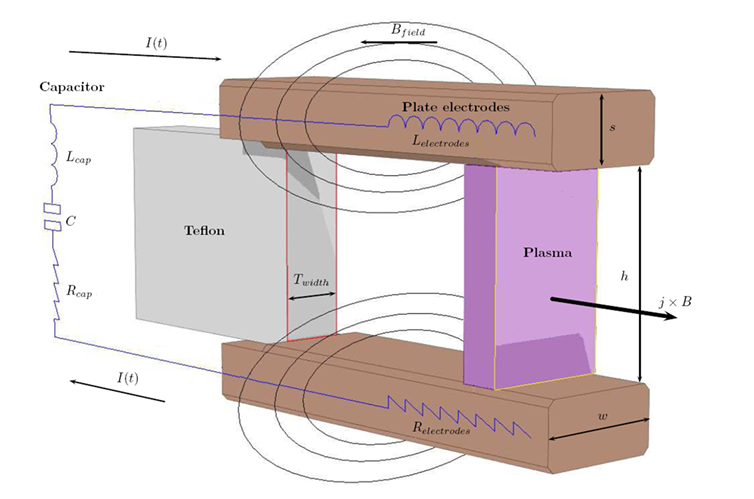
\includegraphics[width=0.8\linewidth]{ppt_circuit_elec.png}
   \caption{Electrical schematic of a PPT  \cite{Shaw_2011} p106}
   \label{ppt_circuit}
\end{figure}


\begin{equation}
V_0 = L \frac{dI}{dt} + RI + \frac{1}{C} \int I\, dt + I\frac{dL}{dt},
\end{equation}

It can be shown using Thomson's theorem that $L_{plasma}$ is negligible \cite{Shaw_2011} p107, and that both $L_{electrodes}$ and $R_{electrodes}$ are small compared to $L_{capacitor}$ and $R_{capacitor}$ \cite{Shaw_2011} p113.

\subsection{Plasma Model}

The plasma is composed of two main regions: the bulk, where the plasma is globally neutral, and the sheath, where positive ions are predominant. As the electric field varies rapidly, electrons are accelerated faster than ions due to their lower mass. It can be shown that the thickness of this region depends on the wall potential $\Phi_{\text{wall}}$, the elementary charge $e$, the vacuum permittivity $ \varepsilon_0$ and the ion density $N_i$ according to \cite{Shaw_2011} p125:

\begin{equation}
d_{\text{sheath}} = \sqrt{\frac{-\Phi_{\text{wall}} \, 2 \varepsilon_0}{e \, N_i}},
\end{equation}

and thus, the current in the sheath can written as a function of the mass of the electron $m_e$ and the surface of the anode $S_{\text{anode}}$:

\begin{equation}
I_{e\text{-sheath}}
= \frac{4 \varepsilon_0}{9}
\left(\frac{2e}{m_e}\right)^{1/2}
\frac{\Phi_{\text{wall}}^2}{d_{\text{sheath}}} S_{\text{anode}}.
\end{equation}

Using a magnetohydrodynamics model, $N_i$ can be determined, while the lumped circuit model provides $\Phi_{\text{wall}}$.
\\[0.5cm]

It can be shown that the flow resistance is negligible compared to that of the sheath. Moreover, if the plasma potential is not too high, the potential of the sheath is approximately equal to the potential of the wall : $V_{\text{sheath}} \simeq \Phi_{\text{wall}}$ \cite{Shaw_2011} p125, and:

\begin{equation}
R_{\text{plasma}} \simeq R_{\text{sheath}} = \frac{V_{\text{sheath}}}{I_{e\text{-sheath}}}.
\end{equation}

\subsection{Equation of Motion}

Using Newton’s second law, the electromagnetic force applied to the plasma flow can be approximated for a rectangular circuit as a function of the width of the electrode $\omega$, the rate of ion erosion $\Gamma_i$, the magnetic permeability of the vacuum $\mu_0$, the current density $J$, the magnetic field $B$ and the distance between the two electrodes $h$  \cite{Shaw_2011} p127 \cite{Grand_2021} p17:

\begin{equation}
\Gamma_i I \frac{dx}{dt} + \Gamma_i \frac{d^2 x}{dt^2} \int_0^t I \, dt = \int_V (J \times B) \, dV=\frac{h\mu_0}{2\omega}I^2=\frac{1}{2}L'I^2.
\end{equation}

\subsection{Performance}

The efficiency of a PPT measures its ability to convert the energy stored in the capacitor into kinetic energy (plasma acceleration). It can be written as a function of the mass of plasma expelled per pulse $m$, the impulse bit (impulse per discharge) $I_{bit}$ and the exhaust velocity $u_e$ \cite{Shaw_2011} p143:

\begin{equation}
\eta = \frac{E_{\text{kinetic}}}{E_{\text{elec}}}
= \frac{\frac{1}{2} m u_e^2}{\frac{1}{2} C V_0^2}
= \frac{I_{bit}}{C V_0}.
\end{equation}


In practical cases, the efficiency is on the order of 10\%. This low value is due to the fact that not all the propellant affected by the electric arc is ionized \cite{Shaw_2011} p145. Moreover, the current in the circuit can be very high (greater than 1 kA), leading to significant Joule losses according to $P = R I^2$.
\\[0.4cm]

The specific impulse of a PPT, $I_{sp} = \frac{u_e}{g_0}$, typically ranges between 250 s and 1400 s \cite{Shaw_2011} p12, depending on the stored energy. This is higher than chemical propulsion but lower than other electric propulsion systems.
\\[0.4cm]

The thrust produced by a PPT is very low (on the order of $\mu N$). For instance, early systems produced around 2 mN with an $I_{sp}$ of 410 s, while more recent systems can reach about $297 \mu N$ with an $I_{sp}$ of 1000 s \cite{Grand_2021} p3.
\\[0.4cm]

One of the main drawbacks of this system is electrode erosion caused by high current densities. For a PPT mounted on a CubeSat, this erosion is on the order of $\mu g$ per discharge \cite{Shaw_2011} p21 (depending on electrode length).

\section{Conclusion}

\subsection{Project Overview}

The study of these five technologies makes it possible to establish a comparative framework based on the analysis of various performance parameters (\cite{rpe_book} p. 622). In accordance with the literature, the most relevant parameters to consider are thrust, which reflects the system’s responsiveness; specific impulse, which indicates efficiency; total propulsion duration; and the power required to generate a unit of thrust.


\begin{table}[H]
    \centering
    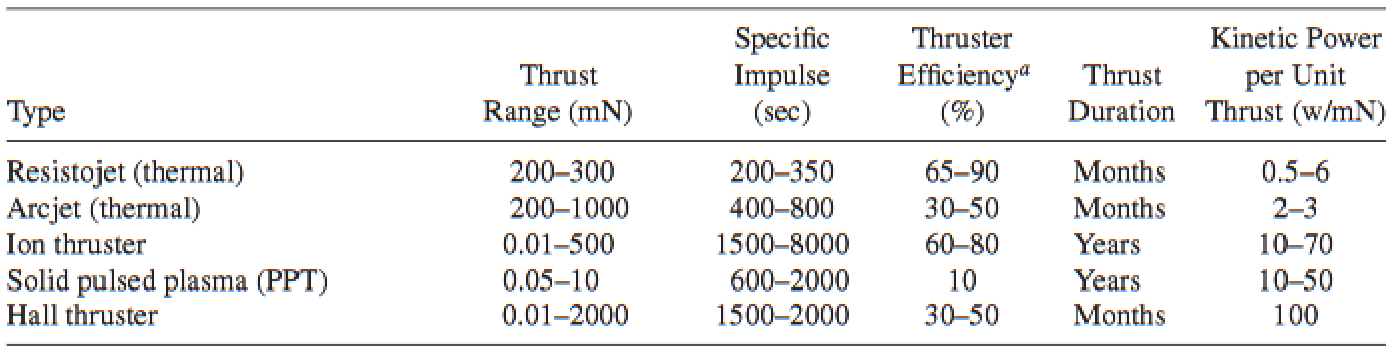
\includegraphics[width=1\linewidth]{figs/tab_recap_vf.png}
    \caption{Performance comparison of the different technologies}
    \label{tab:all_performances}
\end{table}

The selection of a given thruster ultimately depends on a trade-off between mission requirements and operational constraints. It can be observed that electrostatic and electromagnetic technologies generally achieve higher specific impulses—as is the case for ion thrusters—but produce lower thrust levels than electrothermal technologies.
\\

Ion propulsion and Hall-effect thrusters remain the most suitable options for applications that do not require high thrust levels, such as slow orbital maneuvers, station-keeping, or interplanetary and deep-space missions. They offer high specific impulse and superior efficiency compared to alternative electric propulsion technologies.

Conversely, electrothermal propulsion systems, while capable of delivering relatively higher thrust, are less attractive in terms of specific impulse, which remains only marginally higher than that of chemical propulsion systems. In addition, these technologies are subject to significant thermal losses, which further reduce their overall efficiency.

Pulsed Plasma Thrusters (PPT), although technologically advanced, remain limited in efficiency and thrust compared to other electric propulsion systems and is mainly used in small satellites due to their ease of implementation and robustness.
\\

Beyond efficiency considerations, practical factors must also be taken into account when evaluating these different thrusters, such as component erosion and system footprint. From this perspective, Hall-effect thrusters are among the most compact solutions. Ion thrusters and Pulsed Plasma Thrusters (PPT) are also less affected by erosion compared to other technologies (\cite{rpe_book} p. 624).

\subsection{Application Contexts of Electric Propulsion Systems}
This comparison highlights the respective advantages and limitations of each technology, providing a deeper understanding of why certain thrusters are more widely adopted in the industry depending on the application context.

Currently, ion thrusters are predominantly used for GEO satellites and deep-space exploration missions, while Hall-effect thrusters are more commonly employed for LEO and MEO satellites. Arcjet and resistojet technologies also retain relevance for specific applications requiring higher thrust while maintaining a specific impulse superior to that of chemical propulsion. In contrast, Pulsed Plasma Thruster (PPT) technology still faces significant limitations and remains relatively underutilized (\cite{rpe_book} p. 624).

\subsection{Most important things}

This study explores the technical details of electric propulsion and the operating principles of the technologies considered. However, from a broader perspective, it also highlights several general insights into electric propulsion systems. Based on this work, the following presents a non-exhaustive list of the key takeaways regarding electric propulsion:

\begin{enumerate}
	\item There are three main families of physical principles underlying electric propulsion technologies: electrostatic, electrothermal, and electromagnetic thrusters.
	\item Electric propulsion systems provide a higher specific impulse than chemical propulsion but generate significantly lower thrust levels.
	\item Due to their low thrust, electric propulsion systems are not suitable for launch or rapid maneuvers, as they require long operating times to produce significant velocity changes. However, electric propulsion is highly efficient for long-duration maneuvers and orbital corrections, owing to its high specific impulse.
	\item The low thrust levels enable precise control, making electric propulsion well suited for micropropulsion and fine attitude or trajectory adjustments.
	\item The most mature technologies are electrostatic thrusters, particularly ion and Hall-effect thrusters. Other systems, such as resistojets, arcjets, and pulsed plasma thrusters (PPT), still face significant challenges, including limited energy efficiency and electrode erosion.
	\item The primary limitation of electric propulsion is not the availability of propellant, but the available power. This power can be generated from solar energy or supplied by nuclear sources, the latter offering significantly higher energy density than chemical fuels.
\end{enumerate}

In conclusion, the propellant mass required over the lifetime of a spacecraft is significantly higher for chemical propulsion systems:

\begin{center}
\textit{“For NSSK the satellite might need an annual velocity increase of some 50 m/sec; this requires about 750 kg of chemical propellant for the entire period, which is more than one-quarter of the satellite mass. Using an electric propulsion system with a specific impulse of 2800 sec (about nine times higher than a chemical rocket), the propellant mass can be reduced to perhaps less than 100 kg” (\cite{rpe_book} p.625).}
\end{center}

In the context of space systems, every kilogram of mass represents an additional cost, and it is often more beneficial to allocate this mass budget to payload instruments rather than propellant. A quantitative example highlights this advantage:


\begin{center}
\textit{“With launch costs estimated at \$50,000 per kilogram delivered to GEO, this is a potential saving of \$22,500,000 per satellite” (\cite{rpe_book} p.625)}
\end{center}


Electric propulsion systems therefore offer significant practical and economic advantages, which explains their widespread adoption in the space industry today.

As space missions continue to evolve toward longer durations, higher efficiency, and reduced mass constraints, electric propulsion is expected to play an increasingly dominant role. Ongoing advancements in power systems, materials, and plasma physics will likely further enhance the performance and reliability of these technologies, reinforcing their importance in the future of space exploration.

\addcontentsline{toc}{section}{\emph{References}}
\section*{References}

%%% Para usar bibtex:
\bibliography{tex/LE}

\appendix

\section*{Appendices}
\addcontentsline{toc}{section}{\emph{Appendices}}

\section{Contributions}

\begin{table}[H]
\centering
\caption{Individual contributions of each authors}
\label{tab:contributions}
\begin{tabular}{@{}lll@{}}
\toprule
\textbf{Name} & \textbf{Implication} & \textbf{Main contributions} \\ \midrule
Simone Binotto & 95 & Resistojets, Electrothermal thrusters\\
Marco Azevedo & 100 & Arcjets, SW Sensitivity analysis \\
Philippe Quichaud & 100 & Pulsed plasma thrusters, SW Scaling laws \\
Corentin Ouisse & 105 & Hall effect thrusters, SW User interface  \\
Andr\'{e} Matos & 100 & Ion thrusters, SW Scaling and sweeping \\
Th\'{e}o Demesy & 95 & Introduction / Conclusion, Review \\ \bottomrule
\end{tabular}
\end{table}

\section{Software}

The team developped, in addition to this report, a software written in Python that allows the user to dimension an Ion thruster for a given mission. The user can freely specify mission parameters, as for example desired delta-v and payload mass in a text file, but also more specific parameters relative to precise dimensionning of the motor (minimum thrust, component efficiencies, and so on...).

This text file will then be processed by the program which will return an optimal motor design (optimized for mass) described in an output file. It will also provide a table all possible motor configurations encountered in the search process. Finally, it also conducts a sensibility analysis on a specified design objective (eg mass) relative to all mission parameters so that the user can evaluate the effect of design choices.

For further information relative to the software, please refer to the provided README file that explains in detail usage and features.


\end{document}

